\documentclass[a4paper]{amsart}
\usepackage{amsmath, amsthm}
\usepackage{amssymb}
\usepackage{amsfonts}

\newtheorem{thm}{Theorem}[section]
\newtheorem{lem}[thm]{Lemma}
\newtheorem{prop}[thm]{Proposition}
\newtheorem{cor}[thm]{Corollary}
\newtheorem{defn}{Definition}[section]
\newtheorem{example}{Example}[section]
\newtheorem{exercise}{Exercise}[section]
\newtheorem{algorithm}{Algorithm}[section]


\newcommand\be{\begin{equation}}
\newcommand\ee{\end{equation}}
\newcommand\half{\frac{1}{2}}

\newcommand\CC{{\mathbb C}}
\newcommand\EE{{\mathbb E}}
\newcommand\NN{{\mathbb N}}
\newcommand\OO{{\cal O}}
\newcommand\PP{{\mathbb P}}
\newcommand\PPbar{{\overline{\mathbb P}}}
\newcommand\RR{{\mathbb R}}
\newcommand\TT{{\mathbb T}}
\newcommand\ZZ{{\mathbb Z}}

\renewcommand{\theenumi}{(\roman{enumi})}    

\DeclareMathOperator{\conv}{co}
\DeclareMathOperator{\GL}{GL}
\DeclareMathOperator{\Span}{Span}
\DeclareMathOperator{\Vol}{Vol}

\newcommand\fhat{{\widehat{f}}}
\newcommand\ghat{{\widehat{g}}}
\newcommand\Lhat{{\widehat{L}}}
\newcommand\LAhat{{\widehat{L^A}}}
\newcommand\Lhhat{{\widehat{L^h}}}
\newcommand\phihat{{\widehat{\phi}}}
\newcommand\phiAhat{{\widehat{\phi^A}}}
\newcommand\phihhat{{\widehat{\phi^h}}}


\newcommand{\va}{{\bf a}}
\newcommand{\vb}{{\bf b}}
\newcommand{\vc}{{\bf c}}
\newcommand{\vh}{{\bf h}}
\newcommand{\ve}{{\bf e}}
\newcommand{\vg}{{\bf g}}
\newcommand{\vp}{{\bf p}}
\newcommand{\vq}{{\bf q}}
\newcommand{\vu}{{\bf u}}
\newcommand{\vv}{{\bf v}}
\newcommand{\vw}{{\bf w}}
\newcommand{\vx}{{\bf x}}
\newcommand{\vy}{{\bf y}}
\newcommand{\vz}{{\bf z}}

\newcommand{\vL}{{\bf L}}
\newcommand{\vT}{{\bf T}}

\newcommand{\Balpha}{{\mbox{\boldmath $\alpha$}}}
\newcommand{\Bbeta}{{\mbox{\boldmath $\beta$}}}
\newcommand{\Bgamma}{{\mbox{\boldmath $\gamma$}}}
\newcommand{\Bell}{{\mbox{\boldmath $\ell$}}}
\newcommand{\Blambda}{{\mbox{\boldmath $\lambda$}}}
\newcommand{\Bmu}{{\mbox{\boldmath $\mu$}}}

\usepackage{graphicx}
\usepackage{physics}
\usepackage{amsmath}
\graphicspath{ {images/} }

\begin{document}

\title[Multi-Level Sparse Grid Interpolation Kernel Collocation (MuSiKc)]
{The Multi-Level Sparse Grid Interpolation Kernel Collocation (MuSiK-c) Algorithm, Applied to Basket Options}
\author[Nicholas Wilton]{Nicholas Wilton}


\maketitle

\section{Introduction}

Numerical Analysis is the study and use of computation algorithms in approximation within the field of mathematical analysis of which (and in particular interest to this paper), partial differential equations (PDEs) are common throughout many areas of science. Whilst analytic solutions exist for some PDEs using such techniques as 'seperation of variables', 'integral transform' and 'change of variables', often either no solution exists orthe analytic tools are currently insufficient to find it.   

The known algorithms developed for solving PDEs are generally classified into nine main methods:\\
\\
\textperiodcentered Finite Difference\\
Where functions whose known values at certain points are approximated by differences between these values. The grid on which these points (aka. nodes) reside is often referred to as a mesh there each node in a finite difference scheme is connected to it's neighbour in either a forward or backwards manner by the algorithm employed\\
\\ 
\textperiodcentered Method of Lines\\
PDE's in multiple dimensions are discretised into Ordinary Differential Equations (ODEs), in all but one dimension allowing for any of the vast number of numerical integration solvers to be used in these dimensions, meanwhile the final dimension is solved by ...\\
\\ 
\textperiodcentered Finite Element\\
Used for approximating boundary value problems where by the solution is approximated by the composition of many linear elements again using a mesh of nodes connected to each other.\\
\\
\textperiodcentered Gradient Discretisation\\


\textperiodcentered Finite Volume
Similar to both Finite Element and Finite Difference methods, a mesh is created on which values are calculcated at discrete points. Using the diveregence theorem to convert volume integrals into surface integrals around each point...\\
\\ 
\textperiodcentered Spectral\\
Where approximation is done by combining a series of basis functions by superposition and then choosing the co-efficients of the series which minimise the error of the result. For example a Fourier series of sinusoidal waveforms or Radial Basis Functions (RBF).\\
\\ 
\textperiodcentered Meshfree\\
In contrast to the previous methods, which all require connections between nodes of a grid a mesh free method requires no connection between nodes.
\\ 
\textperiodcentered Domain Decomposition\\
Whereby a boundary value problem is split into smaller problems on sub-domains each of which is independent from the others allowing for parallelisation of the overall global problem.
\\ 
\textperiodcentered Multigrid\\
Using a heirachy of descritised grids with different levels of coarseness between the nodes. The idea being that the convergence of an iterative method can be accelerated by solving on a coarser grid to make a global correction to the finer grid.
\\
Recent work by

\section{Theoretical Background}
An in-depth discussion of the theoretical background to this work can be found in \cite{mski0}, whilst here we present a more brief overview of the main points.

\section{Partial Differential Equations}

\subsection{Elliptical PDEs}
If we define a linear operator $L : C^{2} (\Omega) \rightarrow C(\Omega)$ as an elliptic differrential operator on u(x) as:
\begin{equation}
Lu(x) = \sum_{i,j=1} a_{i,j}(x) \pdv{}{x_i}{x_j} u(x) + \sum_{i=1} b_{i}(x) \pdv{}{x_i} u(x) + b_{0}(x) u(x)
\label{EPDE}
\end{equation}
where the coefficient matrix $\big[ a_{ij}(x) \big] \in \Re^{dxd}$ satisfies the condition:
\begin{align*}
\exists \mbox{  } \alpha > 0
\end{align*}
 such that,
\begin{align*}
\sum_{i,j=1}^{d} a_{ij}(x)c_{i}c_{j}\geq \alpha||c||_{2}^{2}
\end{align*}

for all $ x \in \Omega and c \in \Re^{d}$

For a boundary value problem, we would then solve the second order elliptic PDE with the boundary conditions:

\begin{equation}
Lu = f \mbox{ in } \Omega \\
\label{EPDE1}
\end{equation}
\begin{equation}
u = g \mbox{ on } \partial \Omega
\label{EPDE2}
\end{equation}

Where again, L is the elliptic operator and f and g are the functions describing the boundary.

\subsection{Parabolic PDEs}
We can represent parabolic PDEs (for which the Black-Scholes equation is a 2nd order example), in a similar manner. Where L is a linear operator on the domain of $\Omega$ such that:

\begin{equation}
Lu(x,t) = u_{t} \sum_{i,j=1} a_{i,j}(x,t) \pdv{}{x_i}{x_j} u(x,t) - \sum_{i=1} b_{i}(x,t) \pdv{}{x_i} u(x,t) - c(x,t) u(x)
\label{PPDE}
\end{equation}
Which for Black-Scholes in N-dimensions is:
\begin{equation}
LV(S,t) = \pdv{V}{t} + \frac{1}{2} \sum^{d}_{i=1} \sum^{d}_{j=1} \rho_{ij} \sigma_{i} \sigma_{j} S_{i} S_{j} \pdv{V(S,t)}{S_{i}}{S_{j}}+ \sum^{d}_{i=1}(r-q_{i})S_{1} \pdv{V(S,t)}{S_{i}} - rV(S,t)
\end{equation}

To solve parabolic equations with radial basis functions, Zhao uses two methods, The Method of Lines (MoL) and the Space-Time method of Myers incorporating Kansa's approach to elliptical PDEs. A brief overview of the later will be outlined in the next sections whilst a discussion of the former can be found in Zhao's original thesis \cite{}

\subsection{Radial Basis Functions}

A radial basis function (RBF) is a real valued function whose value only depends on the ditance from the origin or centre such that:

\begin{equation}
\phi(x,c) = \phi(||x-c||)
\end{equation}

Where x is the point of interest and $x_{i}$ is the location of the central point. \\Some examples of RBFs are the Euclidean distance:

\begin{equation}
\phi(r) = \sqrt{x^{2} + y^{2}}
\end{equation}
Hardy's Multiquadric RBF:
\begin{equation}
\phi(r) = \sqrt{c^{2} + ||x-x_{i}||^{2}}
\end{equation}

The Gaussian RBF
\begin{equation}
\phi(r) = e^{-||x-x_{i}||^{2} / c^{2}}
\end{equation}

Now, if we want to approximate some function $u(x)$ for a set of scattered data points say $X={x_{1},x_{2},...x_{N}} \subset \Re^{d}$ we would use interpolation via:
\begin{equation}
\hat u(x) = \sum^{N}_{i=1} \lambda_{i} \Phi(||x - x_{i})
\label{RBFA}
\end{equation}
before then solving the linear system:
\begin{equation}
A\lambda =y
\end{equation}
where,
\\ $A_{j,k}= \phi(x_{j}), \mbox{for j,k=1,2,...N}$
\\$\lambda=[\lambda_{1},...\lambda{N}]^{T}$
\\$y=[y_{1},...y{N}]^{T}$
As the inverse of A exists, then we can be sure that a unique solution exists.\\

Of particular interest are the Multiquadric (MQ) and Gaussian RBFs as they are both inifintely differentiable and have been shown to exhibit accuracy, stability and ease of implementation in for example Franke (1982)\cite{rbf3}. As such they have become popular in the literature of various interpolation schemes \cite{rbf4}. In both cases a parameter \em{c} is defined, known as the \em{shape parameter} the size of which will sharpen (decreasing c) or flatten (increasing c) the function.
[TODO insert some graphs]

It has been shown that a larger value of c will increase accuracy but exceed a limit and the system will become ill conditioned and unstable. Likewise reduceing c will improve the conditioning but also lead to an inaccurate solution. There has been significant effort devoted to finding the optimal value of c for different RBFs for example \cite{} however this is still considered an open question within the field.

\subsection Ansiotropic Radial Basis Functions
If the domain of interest is not the same size in all dimensions then an RBF becomes ansiotropic. To model this let $\phi(||\dot -x_{i})$ is some RBF centred around $x_{i} \in \Re^{d}$ and $A \in \Re^{d x d}$ is an invertible transformation matrix, then the ansiotropic radial basis function $\phi_{a}$ is defined by:
\begin{equation}
\phi_{A}(||\cdot-x_{i}||)=\phi(||A(\cdot-x_{i}||)
\end{equation}
Furthermore we can then define the ansiotropic tensor based product function (ATBPF) of the MQ and Gasussian basis functions respectively, as:

\begin{equation}
\phi_{A,x_{i}}(x)= \prod^{d}_{k=1}\sqrt{A^{2}_{k}(x_{k}-x^{k}_{i})^{2}+c^{2}_k}
\end{equation}

\begin{equation}
\phi_{A,x_{i}}(x)= \prod^{d}_{k=1}\exp{\frac{-A^{2}_{k}(x_{k}-x^{k}_{i})^{2}}{ c^{2}_k}}
\end{equation}
Where, k is the $k^{th}$ dimension of x and $A_{k}$ is $k^{th}$ diagonal element of $A \in \Re^{d} x \Re^{d}$.

Whilst we can observe that the Gaussian ATBPF still belongs to the family of RBFs, the MQ ATPBF is no longer radially symmetric.

Now, if we let $Ch_{k} = c_{k} / A_{k}$ we find:

\begin{equation}
\phi_{A,x_{i}}(x)= \prod^{d}_{k=1}\sqrt{(x_{k}-x^{k}_{i})^{2}+Ch^{2}_k}
\end{equation}

\begin{equation}
\phi_{A,x_{i}}(x)= \prod^{d}_{k=1}\exp{\frac{(x_{k}-x^{k}_{i})^{2}}{ Ch^{2}_k}}
\end{equation}

that $Ch_{k}$ represents a 'shape parameter' as noted previously where $h_{k}$ represents the distance between nodes in the kth direction and $A_{k}$ is the number of nodes in that same direction minus one.

The first and 2nd derivtives of the ATPBFs are then in the Mutliquadric case,

\begin{equation}
D_{x_{p}}(\phi_{A,x_{i}})=\frac{x_{p}-x^{p}_{i}}{\sqrt{(x_{p}-x^{p}_{i})^{2} + (Ch_{p})^2 }} \prod^{d}_{k\neq p}\sqrt{(x_{k}-x^{k}_{i})^{2}+Ch^{2}_k}
\end{equation}
\begin{equation}
D_{x_{p}}^{2}\phi_{A,x_{i}}(x)=\frac{(Ch_{p})^{2}}{[(x_{p}-x^{p}_{i})^{2} + (Ch_{p})^2 ]^{3/2}} \prod^{d}_{k\neq p}\sqrt{(x_{k}-x^{k}_{i})^{2}+Ch^{2}_k}
\end{equation}
and in the Gaussian case
\begin{equation}
D_{x_{p}}(\phi_{A,x_{i}})= -\frac{2(x_{p}-x^{p}_{i})}{(Ch_{p})^{2}} \prod^{d}_{k=1}\exp{\frac{(x_{k}-x^{k}_{i})^{2}}{ Ch^{2}_k}}
\end{equation}
\begin{equation}
D_{x_{p}}^{2}\phi_{A,x_{i}}(x)= -(\frac{2}{(Ch_{p})^{2}} + \frac{4(x_{p}-x^{p}_{i})^{2}}{(Ch_{p})^{4}}) \prod^{d}_{k=1}\exp{\frac{(x_{k}-x^{k}_{i})^{2}}{ Ch^{2}_k}}
\end{equation}


It can be shown Zhao Y. (2017) p25-26 \cite{mski0} that for higher dimensional problems we can use the tensor product of ATBPFs to find:

\begin{equation}
(\Phi^{-1}=(\Phi_{1})^{-1} \otimes ... \otimes  (\Phi_{d})^{-1} )
\end{equation}

\begin{equation}
\lambda = (\Phi)^{-1} \cdot y
\end{equation}

Here, Zhao makes some important points:
Inverting $\Phi$ matrix would cost $O(N^{6d})$
For $\Phi{i}$ this becomes $O(N^{6})$
and the Kroencker Product is $O(N^{2d})$

Therefore potentially using ATPBFs produces some good performance benefits over and above summing RBFs when scaling in multiple dimensions.

Whilst Zhao also discussed convergence he also notes there is no current theoretical proof of the convergence of MuSiK-c however his numerical experiments do demonstrate that it does.

\subsection{Kansa method}

Kansa's method \cite{rbf1} \cite{rbf2} is a spectral method of approximating u(x) via:

\begin{equation}
\hat u(x) = \sum^{N}_{i=1} \lambda_{i} \Phi(||x - x_{i})
\label{RBFA}
\end{equation}

Where $\Phi$ is the radial basis function of choice.

For Kansa's method we choose a $\Xi = \Xi_{1} \cup \Xi_{2}$ which we will call central nodes and where $\Xi_{1} \in \Omega$ (i.e are interior points) whilst  $\Xi_{2} \in \partial \Omega$ exist on the boundary $\partial \Omega$

The key of course, is to find the $\lambda$ coefficients for each of the summation terms that make the best approximation of the function u(x). For the elliptical PDE of (\ref{EPDE}) we can substitute (\ref{RBFA}) into the boundary counditions (\ref{EPDE1}) and (\ref{EPDE2}) to get:

\begin{equation}
\sum_{i=1}^{N} \lambda_{i} L \phi_{x_{i}}(x_{j}) = f(x_{j}),\mbox{for j = 1,2,...n}
\end{equation}

\begin{equation}
\sum_{i=1}^{N} \lambda_{i} \phi_{x_{i}}(x_{j}) = g(x_{j}),\mbox{for j = n+1,n+2,...N}
\end{equation}

Which as a matrix system can be represented as:


\begin{align*}
\begin{bmatrix}
 L \phi_{A,x_{1}}(x_{1}) &L \phi_{A, x_{2}}(x_{1}) &... &L \phi_{A, x_{N}}(x_{1})\\
 L \phi_{A, x_{1}})(x_{2}) &L \phi_{A, x_{2}}(x_{2}) &... &L \phi_{A, x_{N}}(x_{2})\\
\vdots &\vdots &\vdots &\vdots\\
 L \phi_{A, x_{1}})(x_{n}) &L \phi_{A, x_{2}}(x_{n}) &... &L \phi_{A, x_{N}}(x_{n})\\
 \phi_{A, x_{1}})(x_{n+1}) &\phi_{A, x_{2}}(x_{n+1}) &...  &\phi_{A, x_{N}}(x_{n+1})\\
\vdots &\vdots &\vdots &\vdots\\
 \phi_{A, x_{1}})(x_{N})  &\phi_{A, x_{2}}(x_{N}) &...  &\phi_{A, x_{N}}(x_{N})
\end{bmatrix}
\begin{bmatrix}
\lambda_{1}\\
\lambda_{2}\\
\vdots\\
\lambda_{n}\\
\lambda_{n+1}\\
\vdots\\
\lambda_{N}
\end{bmatrix}
=
\begin{bmatrix}
f_{1}\\
f_{2}\\
\vdots\\
f_{n}\\
g_{n+1}\\
\vdots\\
g_{N}
\end{bmatrix}
\end{align*}


Whilst much work using collocation with RBFs had been performed using Kansa's method to solve elliptic boundary value problems, it wasn't until Myers et al. \cite:{rbf0} proposed the space time method that applications for parabolic problems were first successfully investigated.


\subsection{Myer's Space-time method}

In a parabolic problem with a have a spacial domain $\Omega \in \Re^{d}$ and a time domain $t \in [a,b]$ if we let $\Omega_{t} = \Omega x t \in \Re^{d} x [a,b]$ then $\pdv{\Omega_{t}}$ represents the portion of $\Omega_{t}$ that is the boundary.
If the centre nodes $\Theta \in \Omega_{t}$ and $\Theta = \Theta1 \cup \Theta2$ then $\Theta1$ are the nodes in $\Omega_{t}$ excluding $\pdv{\Omega_{t}}$ and $\Theta2$ are the nodes on the boundary $\pdv{Omega_{t}}$. As with the elliptical PDE, we can show our boundary value problem as:
\begin{equation}
L_{t} = f, within \Omega excluding \pdv{\Omega_{t}}
\end{equation}
\begin{equation}
u = g, on \pdv{\Omega}
\end{equation}
In this case $L_{t}$ is the parabolic operator whilst f and g are the boundary functions that ensure u satisfies the PDE.

As with the elliptical problem \ref{}, we can now use Kansa's method to solve this system


\subsection{Spectral Methods and the Gibbs phenomena}
Describe issues with Gibbs phenomena



\subsection{Finite Difference}

\subsection{Method of Lines}
Describe how combinationation technique of MoL reduces Gibbs problem

\subsection{Sparse Grid Collocation}

As we have seen in \ref, it is relatively easy to use RBF interpolation in higher dimensions, but as mentioned in \ref{} the distance between nodes must be fixed in order to maintain accuracy. Therefore as the number of dimensions increases, the number of nodes (and hence the number of computations) increases proprotionally to $N^{d}$ where N is the number of equi-distant points in the mesh. This phenomena is sometimes refered to as the curse of dimensionality, the concept that either the amount of computation or the space requirements of an algorithm increase exponentially with the number of dimensions.

Whilst the original ideas around Sparse grid Interpolation Kernels (SiK) originated in the Soviet Union\cite{sik1}\cite{sik2} during the 1960s, it wasn't until Zenger (1991) \cite{sik3} work that the use of sparse grids in PDE solvers really gained traction. Zenger's method relies on the ideas set out in \ref{} ATRBF to save large amounts of space and computation.






\section{Implmentation Details}
The implementation of the algorithmns described above was originally written in MatLab with parrallel extensions for CPU processing and unfortunately only computes solutions to 1-dimensional (i.e. single asset) european call options. In order to expand this codebase (further more refered to as cMuSiK.m) to handle multiple dimensions and scale the available processing power across CPUs and GPUs a two step strategy was undertaken.

1. Convert the MatLab code into C++
2. Convert the C++ code into CUDA C++

As C++ is a versatile multi-paradigm language with good performance capabilities, we can be relatively confident of improving both the maintainability of the codebase whilst keeping the performance without having to micro-optimise. Additionally C++ is sufficiently close to the native language of NVidia's CUDA that the transition from step-1 to step-2 should be relatively easy. Also the available skills base for C++ is quite high, meaning that the resulting codebase should be easier for others to understand and improve.

For the purposes of step-1 C++12 was used primarily for it's in built support for threading and the environment of Microsoft's Visual Studio 2017 due to the familiarity of the author and it's availability as a free toolset. Care was taken to ensure no platform specific libraries were used such that compilers other than Microsoft's implentation should easily be able to compile the codebase given an appropriate build system. The resulting Visual Studio Solutions, a mixed C++ and CUDA implementation (refered to as SparseGridCollocation.sln) and a pure C++ implementation (referred to as SparseGridCollocationCPP.sln) are the results of this conversion process.

In both solutions the code is generally arranged within namespaces and seperated into sub-projects:
Leicester
	SparseGridCollocation
		ProjectSpecific

Specific functions and classes within the solution will be referred to by the Namespace::Class::Function convention for example, Leicester::SparseGridCollocation::Algorithmn::MuSiKc() refers to the main entry point of the MuSiKc implmentation, whilst Leicester::Common::printMatrix() refers to a particular helper function that prints the contents of a matrix to a string.

Each subproject will compile into a seperate dynamically linked library (.dll) or an executable program (.exe). For C++ specific code (i.e. projects containing files with extensions .cpp and .h) the msvc compiler will perform the compilation and linking whilst CUDA specific projects (extensions .h or .cuh and .cu) are handled by the NVidia nvcc compiler. Details of both these compilers and their respective software development kits (SDKs) can be found within the appendix.

\subsection{Reverse Engineering via Unit Testing}
A common method known within the software engineering community to reverse engineer computer programs who's source code is unavailable is the process of black-box unit testing \cite{unit testing}. This is the process of treating the program as a 'black-box' where the actual functionality of a particular program can be revealed by carefully selecting the input to the program and measuring the resulting out puts. For example if we input the full range of integers into a black-box and observe the results to be squares of the input then we can be reasonably confident that the program implements $F(x) = x -> x^{2}$

Whilst in our case the source code is available, this technique can still provide us with a method of measuring and detecting any difference in functionality between our new C++ code and that of the original MatLab code.

SparsGridCollocation.sln and MuSiKc.m include a number of methods and frameworks in order to isolate particular modules of functionality some of which are:
Leicester::SparseGridCollocation::checkMatrix() - Of which there are 3 versions, allowing the user of the function to compare with configurable precision, the sameness of 2 matrices.
Leicester::Common::Utility::printMatrix() - Including several variants that will write the contents of a matrix to a string in various formats prior to inserting into cout and printing to the console
Leicester::Common::Utility::saveMatrix() - Save the contents of a matrix to a human readable text file
Leicester::Common::Utility::saveMatrixB() - Save the contents of a matrix to a binary file so as not to lose precision but the dimensions of the matrix are not saved.
WriteAllToFile.m - Save the contents of a matrix to a binary file.
TestHarness.vcxproj - Contains a simple console application to use as a workbench for running various functions and comparing their output.
Microsoft Test Frame work -  The UnitTest.csproj contains a number of unit tests that when executed within Visual Studio will run parts of or the entire algorithmn of choice with a standard input and check the actual output against an expected output


\subsection{Eigen API and MatLab comparison}
Eigen styles itself as a 'C++ template library for linear algebra: matrices, vectors, numerical solvers, and related algorithms.' which is open source and distributed under an MPL license. What makes this particular library stand out from others is its coverage of MatLab functions. In particular Zhao makes use of the following MatLab functionality that Eigen also replicates:
Linspace - create a linearly spaced vector within a range for a certain number of points
zeros, ones and fill
size
Column \& Row addressing
row wise and column wise sum
Meshgrid
LU decomposition
LU Solver

\subsection{Column Major Format}
There are two main methods for representing a Matrix within computer memory row-major and colmn-major formats. With both, each element within the matrix is mapped to an element within contiguous memory. The difference between them however is the exact mapping between those rows and columns and the consecutive elements within memory. It is therefore worth descibing in some detail the exact differences and the convention used here.

An array of values (for example the values 1,2,3...n) are normally stored as consecutively at equally spaced addresses within computer memory, this is known as contiguous memory. If the first element is stored at address A and the size of each value is x, then for element n within an array of length N, the nth element is stored at A + (x * n).

<<insert image contiguous arrays >>

In row-major format each row is appended to the array, with each row element at consecutive loactions

\begin{figure}[h]
\centering
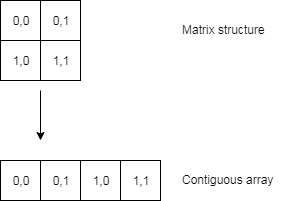
\includegraphics[scale=0.5]{RowMajorFormat1.png}
\caption {Row Major Format}
\label {fig:rowmajor}
\end{figure}


In column- major format each column element is at a consecutive location, while each column is proceedingly appended to the end of the array

<< insert image col-major>>

The convention used within this project is column-major format, which is the same method as both the Eigen library and that of MatLab. Unfortunately the array construct in C and C++ is simply a pointer to the first element and no further information is provided. Consequently unless the dimensions of an array are known at compile time, for example:

int m[] = int[10]; 

or unless the programmer stores the dimensions of a dynamic array:

int rows =10;
int cols = 10;
int *m = int[rows*cols];

it is impossible to reconstruct the array or matrix from contiguous memory which has big implications that we will see in section \ref{cuda}


\subsection{Expressions and Lazy Evaluation}

Another advantage of Eigen is a useful optimisation for handling wasteful processing called expression trees, which as a concept are similar to those seen in C\# LINQ or SQL. Designed to reduce the number of repeated parsings of a Matrix or array by the programer, Eigen 'records' at compile time all operations performed on a particular matrix and constructs an 'expression' representing the aggregate.Eigen then generates the optimal code to perform the aggregate operation on the matrix in as few loops as possible. Eigen will often do this as late as possible and when done so at actual runtime is known as Lazy Evaluation.

For example, say the programer wanted to add a constant to each element of a Matrix and then later on in the program square each element they might write:


Matrix m = Ones::(rows, cols);\\
int c = 1;\\
\t for (int i =0; i < rows; i++)\\
	for (int j =0; j < cols; j++)\\
	{\\
		m(i,j)	+= c;\\
	}\\
.\\
.\\
.\\
for (int i =0; i < rows; i++)\\
	for (int j =0; j < cols; j++)\\
	{\\
		m(i,j)	*= m(i,j);\\
	}\\
\\


In this example it is easy to see that each element of the matrix 'm' is visited by the program twice, but this is obviously wasteful when one considers the following:\\

Matrix m = Ones::(rows, cols);\\
int c = 1;\\
for (int i =0; i < rows; i++)\\
	for (int j =0; j < cols; j++)\\
	{\\
		int a  = m(i,j)	+ c;\\
		m(i,j) = a * a;\\
	}\\

Where a more efficient programmer will realise that each element of 'm' only needs to be visited once by the program. Eigen's expressions perform the same kind of optimisation when working with Eigen's Matrix template classes, freeing the programmer to concentrate on writing functioning code rather than manually optimising that code.

\subsection{Intel Math Kernel Library}
All the algorithmns studied within this paper make use of some linear algebra and MuSiK-c in particular uses vector-vector, vector-matrix, matrix-matrix (i.e. BLAS levels 1-3) and LAPACK routines for decomposition and solving linear systems.

Whilst it is possible to use Eigen without any further dependency, it is recommend that instead of using it's inbuilt support for BLAS and LAPACK it is best to use a platform specific provider. In our case, we have chosen Intel Math Kernel Library\cite{mkl1} (MKL) which is optimised for Intel based chips\cite{mkl2} and their SSE\cite{mkl4}, SSE2 and SSE3 instructions sets for Single Instruction, Multiple Data\cite{mkl3} (SIMD)

Briefly, SIMD allows the processor to stream multiple datasets onto a CPU core in parallel during one instruction. A core is in essence an independent processing unit and modern CPUs are designed to have several of these all on the same chip. What this means is that the same operation can be performed at the same time on several pieces of data simultaneously. Without SIMD that single instruction would need to be executed in serial on each data element individually, which is clearly a vast improvement.

This is particularly useful when used in conjunction with multiple threads operating on a multi-core CPU. Each thread of execution operating on a per core basis can process large data sets themselves in parallel giving us effectively two layers of parallelisation.

%Both versions of the SparseGridCollocation solution are compiled with the directive EIGEN_USE_MKL_ALL in order to enable useage of MKL, please see the supporting documentation for further reference.


\subsection{Parallelisation with C++ Threading and CUDA}

Whilst one of the main goals of this paper is improve the performance of MuSiK-c via parallelisation, it is important to note that not all algorithmns are can take advantage of such improvements. So firstly, we will explain what we mean by parallelisation and also explore some examples that are inherently sequential. 


Secondly we will detail which parts of MuSiK-c are able to take advantage of these techniques. 


Thirdly, how Nvidia's CUDA achieves massive parallelisation and how CUDALib.vcxproj implements some simple parallel routines.

NVidia GPU Hardware architecture

GPU hardware differs some what from that of CPU architecture figure \ref{fig:CPUGPU} shows how a GPU packs far more cores on to chip than does a CPU. Cores are organised into Streaming Multiprocessors (SM) aka a Warp the GPU equavalent of a CPU's SIMD enabling parallelisation of data flow into and out of the GPU.

\begin{figure}[h]
\centering
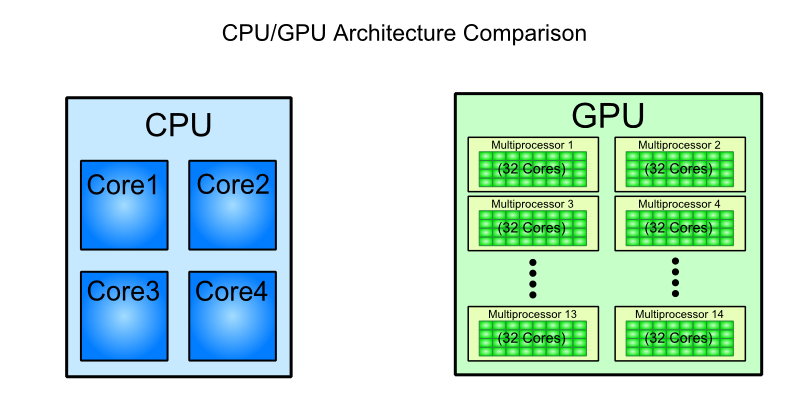
\includegraphics[scale=0.5]{cpu_vs_gpu-1.png}
\caption {CPU vs GPU Architecture}
\label {fig:CPUGPU}
\end{figure}

Whilst it might seem from this that GPUs are far superior to CPUs where the are lacking is in the amount of RAM the GPU cores can access. For example the reference hardware in \ref{refhardware} is a current (as of 2017) GPU containing 2Gb of memory, whereas the CPU (a 2011 vintage) can access the entire 16 Gb of system RAM with ease.

CUDA's threading model is shown in figure \ref{fig:CUDAthread} on page \pageref{fig:CUDAthread} and like all concurrent execution models, the unit of execution is known as a thread but in CUDA threads are also organised using Blocks and Grids.
\begin{itemize}
  \item Thread: A unit of sequential execution, in CUDA all threads execute the same sequential program in parallel.
  \item Thread Block: A group of threads which all execute on the same streaming multiprocessor. Threads within a block can synchronise with each other and exchange data.
  \item Grid: A group of Thread Blocks where blocks execute across multiple SMs, can't synchronise and communication between is expensive.
\end{itemize}

The CUDA runtime API provides a thread ojbect that allows the programmer to identify the x-y-z 3-dimensional coordinate of the thread within it's block as well as the same data for the block within the grid.

\begin{figure}[h]
\centering
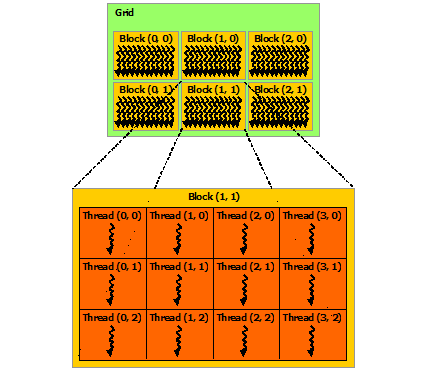
\includegraphics[scale=1.0]{grid-of-thread-blocks.png}
\caption {CUDA threading model}
\label {fig:CUDAthread}
\end{figure}


Initally, it seems that CUDA is designed specifically for our purposes: parsing large NxM matrices in parallel. As we can keep track of the Thread's x and y indices within the larger grid and block   system we launch a grid with enough blocks and threads to process each element of the matrix in parallel. Likewise as the most efficient method is to use blocks of 32x32 threads we can launch more threads than we need but let some 'out of index' threads process nothing.

In general a CUDA program's functions are organised into 3 main types based on whether they are executed on the host-side (the CPU) or the device-side (the GPU):

\begin{itemize}
  \item Kernel: What is termed as the host-side program i.e. operates as a normal C++ program on the CPU able to address system memory and call the Cuda Runtime API
  \item Global Functions: A device-side function that can be called from the Kernel but also from other device-side functions. These functions must be executed by defining grids, blocks and threads that will execute the function concurrently.
  \item Device Functions: Functions that can only be called by device side code and as such themselves run on the device. As with Global Functions must be executed with a declared set of threads.
\end{itemize}

The CUDA runtime is rather limited, in that useful libraries such as the C++ Standard Template Library (STL) or Eigen are not useable on the GPU. Furthermore the runtime only supports the copying of data from host to device (or device to host) via the use of pointers. Both of these drawbacks present significant problems to the programmer. A matrix therefore must be represented by a pointer construct (hence our explanation or column-major format in \ref{}) in order to be loaded by the GPU and passed across functions. Likewise once copied back to the host the pointer array must be mapped back to a matrix structure. For MuSiK-c this means that our dynamically sized matrices are difficult to handle correctly in CUDA unless we pass the dimension sizes around with them. This also complicates (very significantly) the implementation of our grid interpolations as we must keep track of different indes pointing to different elements in our Test Nodes and our Central Nodes.

To add further complexity to the mix, imagine you wanted to execute a grid with n blocks of m threads but each thread itself had to spawn another grid of p blocks and q threads. CUDA can do this as well via what it calls 'Dynamic Parallelism' an example of which can be seen in CudaLib.vcxproj where $CudaLib::Gaussian2d_CUDA$ launches $CudaLib::Gaussian2d2_CUDA$. Dynamic Parallelism is important for applications such as MuSiK-c where there are at least two layers that can be parallelised i.e. ShapeLambda and RBF Interpolation. The big drawback is that without multiple graphics cards installed on your system, it is not possible to debug these kinds of routines. 

As a result of the difficulty in indexing dynamically sized matrices in contiguous memory and that the reference hardware only included one CUDA capable GPU, CudaLib works reasonably well for 1 dimensional european call options at low levels. However not so for the larger matrices encountered at level 7 and above or for Basket options.


\subsection{CUDA Thrust Library}

CUDA Thrust is an abstraction over the main CUDA programming model. It in effect allows the user to define their matrices in an STL-like vector container, define a special function called a 'functor' and the thrust library will automatically copy the matrix to the GPU and execute the functor against every element in the matrix. What is especially useful in our case is that the functors are stateful, such that they are defined as a C Struct type allowing us to know within the function body the dimensions of the various matrices that we are processing as well as any further supporting data we may wish to access.







\section{Algorithm Details}

\subsection{SiK-c}
The basic Sparse Grid Col-located Interpolation Kernel (SiK-c)

N- matrix

\subsection{MuSik-c}
MuSiKc on the otherhand use multi-level co-located interpolation, where the results of each level are re-used as inputs for the next. As such, MuSiK-c is an inherently sequential evolution of SiKc.\\
 The following diagram shows the processing flow of the algo.\\

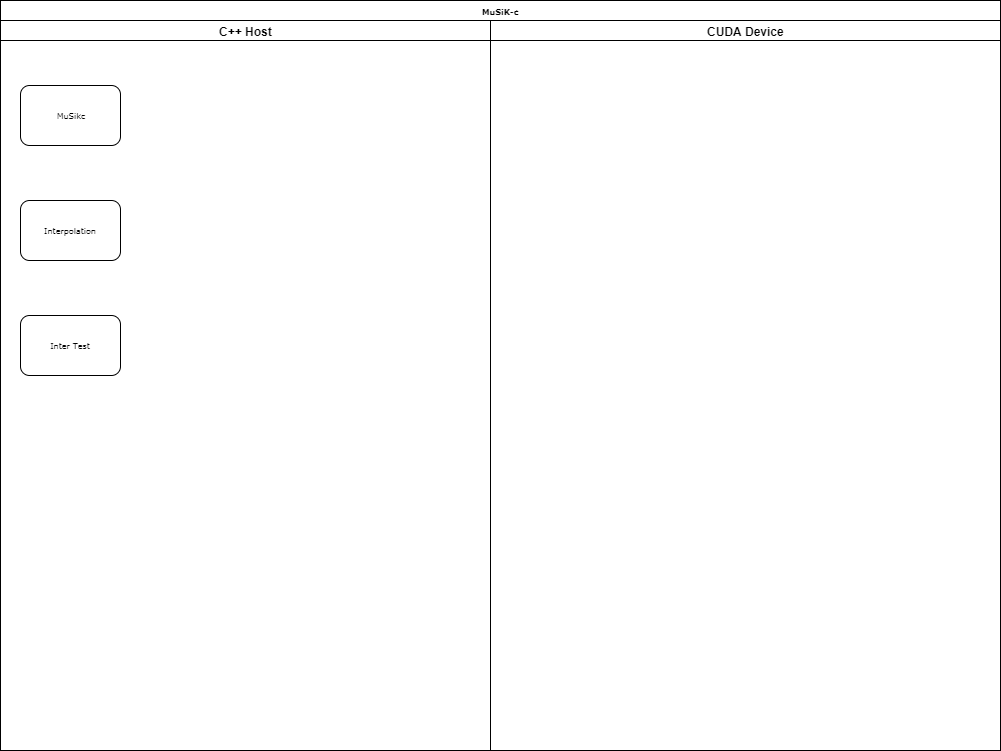
\includegraphics[scale=0.3]{MuSiKc1.png}

\subsection{Computational Complexity Comparisons}

 


\section Computational Experiments



\section Conclusions

\section Further Work

\section{Appendices}

\subsection{Code Repositories}

\subsection{Supporting Documents}
 





\begin{thebibliography}{99}
\bibitem{mski2} Georgoulis, E.h., Levesley, J., Subhan, F. (2013), {\em Multilevel sparse kernel-based interpolation}, SIAM Journal on Scientific Computing, 2013, 35(2):A815-A831.
\bibitem{mski1} Subhan, F. (2011), {\em Multilevel sparse kernel-based interpolation}, Ph.D. Thesis, University of Leicester, 2011.
\bibitem{mski0} Zhao, Yangzhang (2017), {\em Multilevel sparse grid kernels collocation with radial basis functions for elliptic and parabolic problems}, Ph.D. Thesis, University of Leicester, 2017.
\bibitem{rbf0} Myers, D.e.,De Iaco, S.,Posa, D.,De Cesare, L. (2002), {\em Space-time radial basis functions}, Computers and Mathematics with Applications 2002 43(3):539-549
\bibitem{rbf1} E. J. Kansa. (1990), {\em Multiquadrics - a scattered data approximation scheme
with applications to computational fluid-dynamics - I.}, Computers and Mathematics with Applications, 19(8-9):127–145, 1990.
\bibitem{rbf2} E. J. Kansa. (1990), {\em Multiquadrics - a scattered data approximation scheme
with applications to computational fluid-dynamics - II.}, Computers and Mathematics with Applications, 19(8-9):147–161, 1990.
\bibitem{rbf3} R. Franke. (1982), {\em Scattered Data Interpolation: Tests of Some Method}, Mathematics of Computation. 38(157):181-200, 1982
\bibitem{rbf4} A. Pena. (2005), {\em Option pricing with radial basis functions: a tutorial.} Technical
report, Wilmott Magazine, 2005.
\bibitem{sik1} K. I. Babenko. (1960), {\em Approximation by trigonometric polynomials in a certain class of periodic functions of several variables} Soviet Mathematics Doklady, 1:672–675, 1960.
\bibitem{sik2} S. A. Smolyak. (1963), {\em Quadrature and interpolation of formulas for tensor product of certain classes of functions.} Soviet Mathematics Doklady, 4:240–243, 1963.
\bibitem{sik3} C. Zenger. (1991), {\em Parallel algorithms for partial differential equations.} Notes Numerical Fluid Mechanics Vol 31 pages 241-251. Vieweg, Braunschweig, 1991.

\bibitem{mkl1} Intel (2017), {\em Developer Reference for Intel Math Kernel Library} https://software.intel.com/en-us/mkl-developer-reference-c
\bibitem{mkl2} Intel (2017), {\em Intel Streaming Extensions Technology} https://www.intel.co.uk/content/www/uk/en/support/processors/000005779.html
\bibitem{mkl3} Wikipedia (2017), {\em SIMD} https://en.wikipedia.org/wiki/SIMD
%\bibitem{mkl4} Wikipedia (2017), {\em Streaming SIMD Extensions} https://en.wikipedia.org/wiki/Streaming_SIMD_Extensions

\bibitem{cuda1} Nvidia (2017), {\em Memory Optimizations, CUDA C Best Practices Guide} http://docs.nvidia.com/cuda/cuda-c-best-practices-guide/index.htm

http://docs.nvidia.com/cuda/
%http://docs.nvidia.com/cuda/cuda-c-programming-guide/index.html#programming-model
%http://docs.nvidia.com/cuda/cuda-c-programming-guide/index.html#memory-hierarchy
%http://docs.nvidia.com/cuda/cuda-c-programming-guide/index.html#heterogeneous-programming
%http://docs.nvidia.com/cuda/cuda-c-programming-guide/index.html#hardware-implementation
%http://docs.nvidia.com/cuda/cuda-c-programming-guide/index.html#c-language-extensions
%http://docs.nvidia.com/cuda/cuda-c-programming-guide/index.html#cuda-dynamic-parallelism
%http://docs.nvidia.com/cuda/cuda-c-programming-guide/index.html#c-cplusplus-language-support
%http://docs.nvidia.com/cuda/cuda-c-programming-guide/index.html#standard-library

http://docs.nvidia.com/cuda/thrust/index.html






\end{thebibliography}



\end{document}





